\chapter{System Perspective}

\section{System Design}
The present MiniTwit system represents a refactored and optimized version of the of the legacy codebase that was originally provided. The present system is organized into three distinct components, including a \textit{C\# ASP.NET} project that functions as the \textit{backend component}, a \textit{React-based frontend} component, and a \textit{NoSql mongoDB database}. These particular technologies were selected on the basis of the developers existing familiarity with these tools, which has been achieved from prior courses and practical experience. 

\begin{figure}[H]
    \centering
    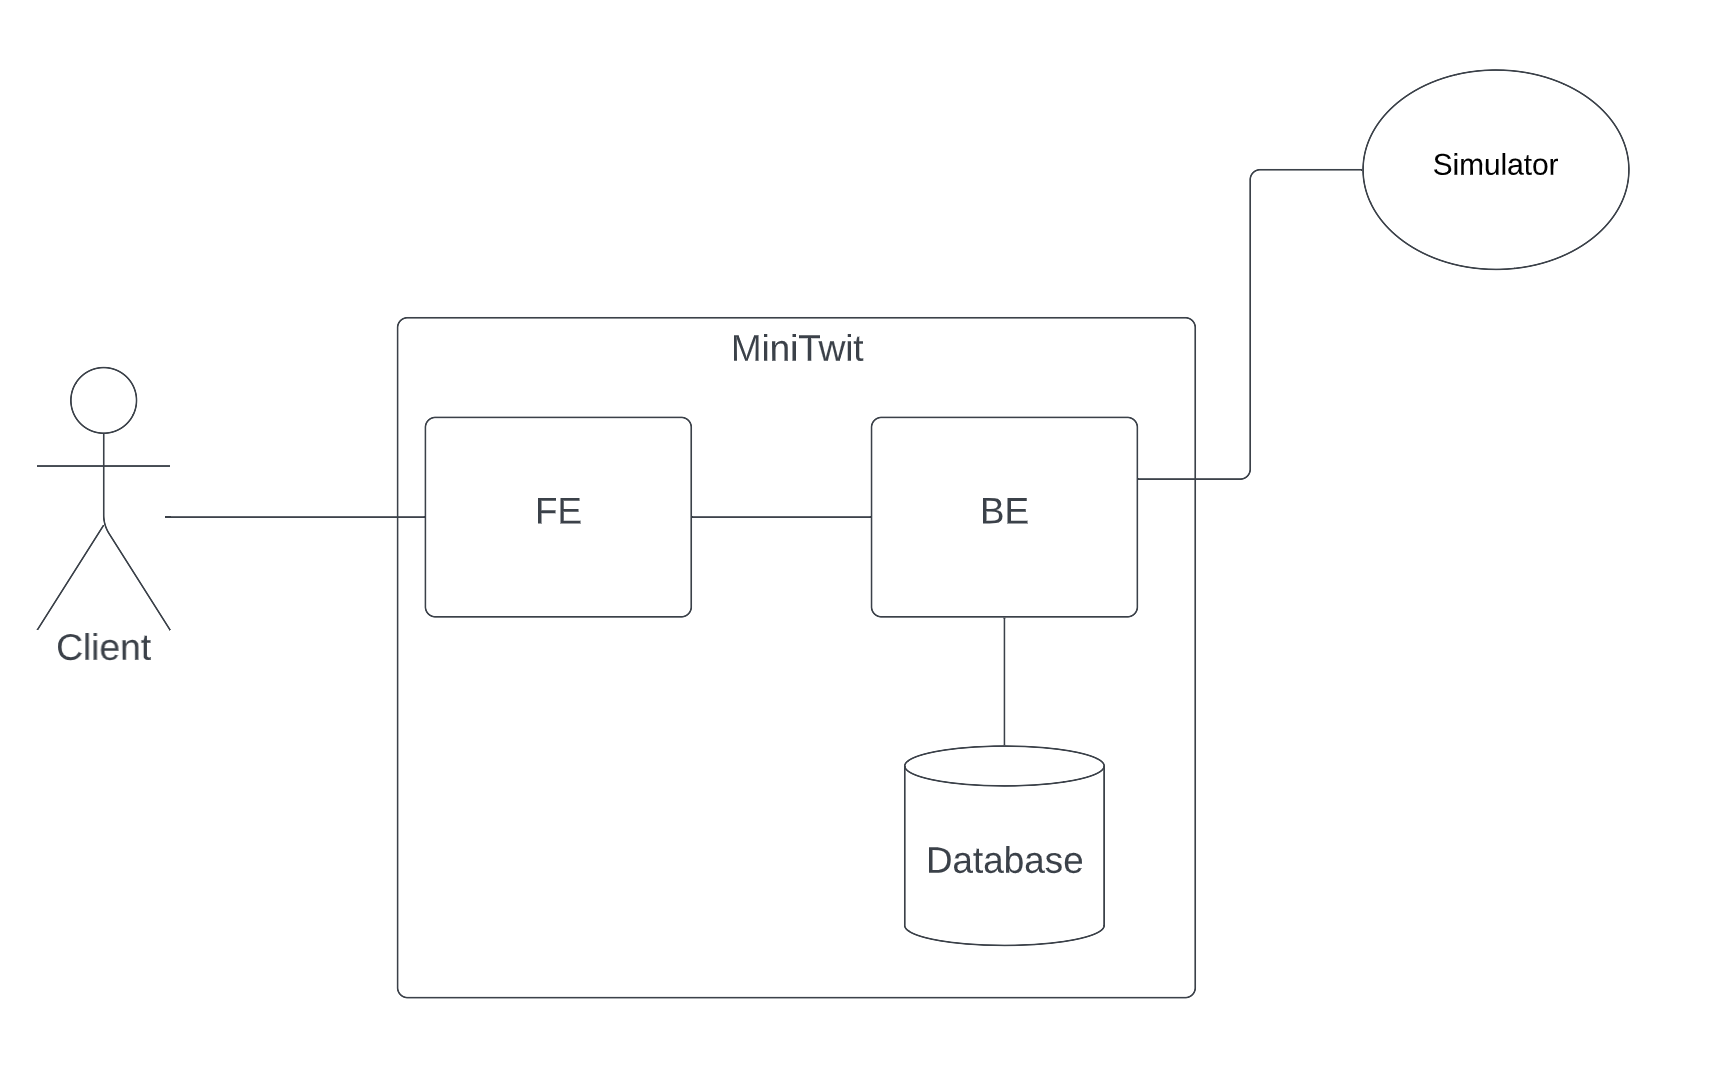
\includegraphics[width=12cm]{Use_case.png}
    \caption{System Design (use case)}
    \label{fig:use_case_diagram}
\end{figure}

We quickly decided to create all services as docker images, to avoid having seperate local build scripts as we develop on different OS.


\begin{figure}[H]
    \centering
    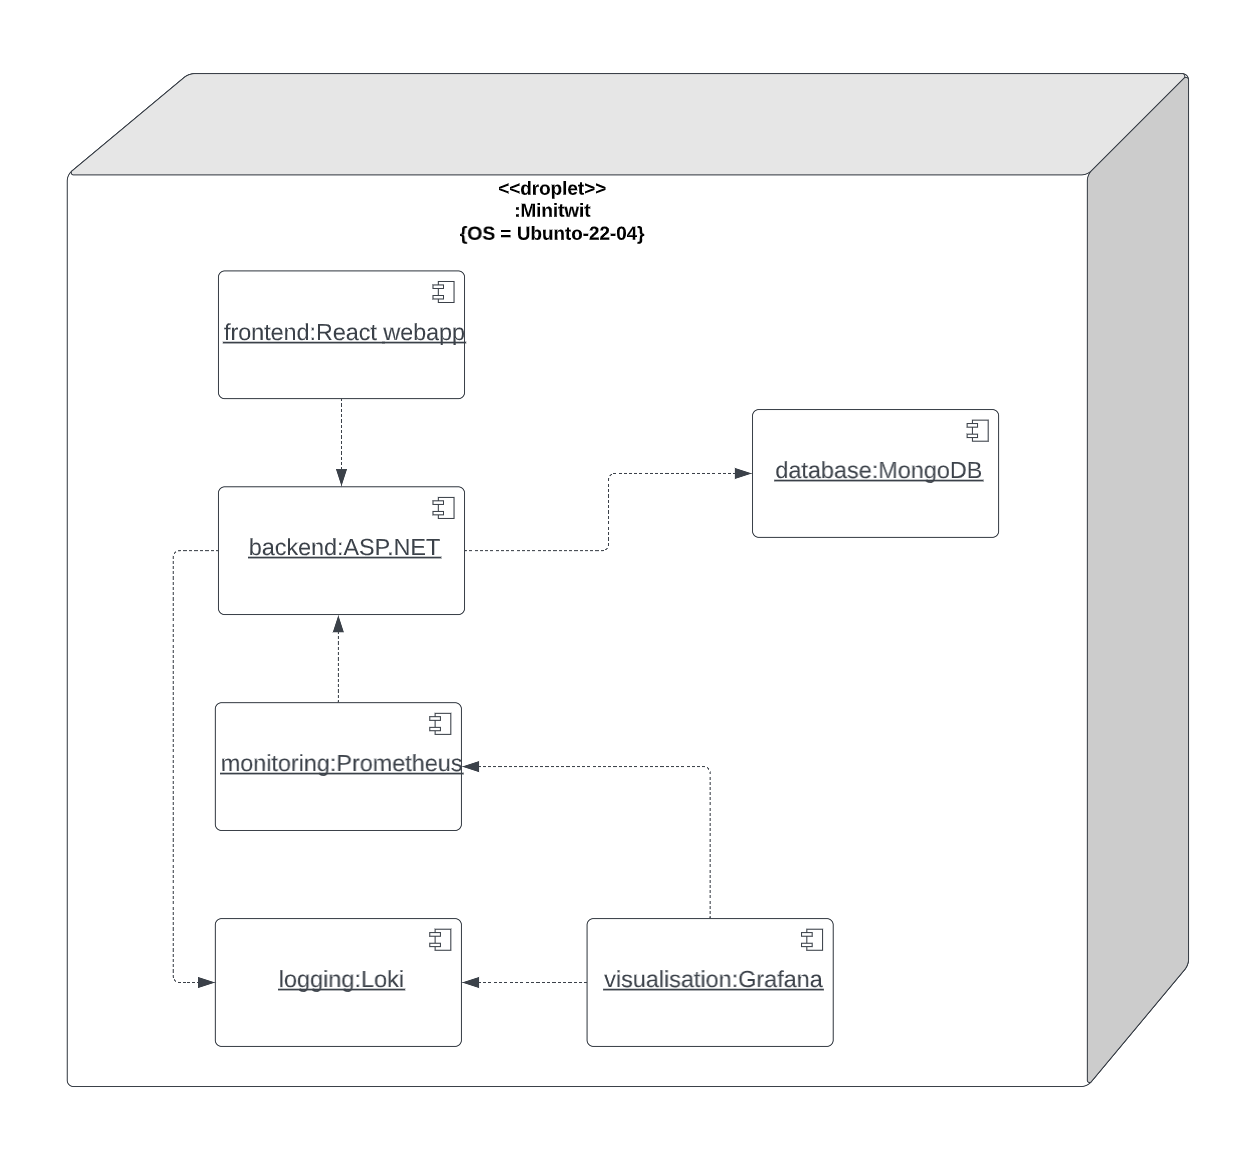
\includegraphics[width=12cm]{deployment_diagram.png}
    \caption{Minitwit deployment diagram}
    \label{fig:deployment_diagram}
\end{figure}

\section{System Architecture}

\subsection{Subsystems} \label{sec:subsystems}

\subsubsection{MiniTwit Backend}

The \texttt{MiniTwit} backend was designed according to the Onion Architecture which is based on the Inversion of Control principle. The architecture is comprised of multiple concentric layers that interface with each other toward the core. The flow of dependency, therefore, goes inwards making it easy to test and maintain each layer, as the coupling is low.

The backend is split into four layers and five separate C\# projects (see figure \ref{fig:backend-onion}):

\begin{enumerate}
    \item Domain Layer (MiniTwit.Core): Contains the domain models
    \item Infrastructure Layer (MiniTwit.Infrastructure): 
    \item Service Layer (MiniTwit.Service \& MiniTwit.Security)
    \item Presentation Layer (MiniTwit.Server)
\end{enumerate}

\begin{figure}[H]
    \centering
    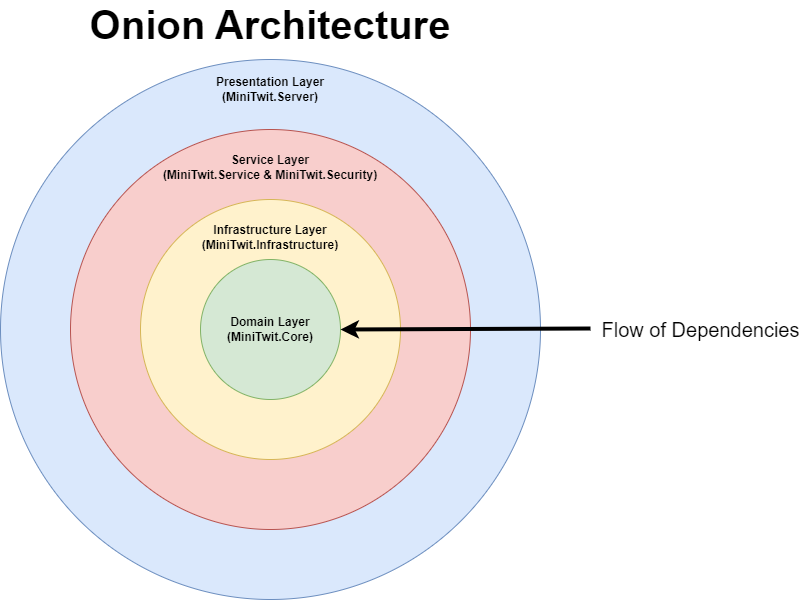
\includegraphics[width=\linewidth]{architecture/minitwit_onion.png}
    \caption{The Onion Architecture of the \texttt{MiniTwit} backend.}
    \label{fig:backend-onion}
\end{figure}

\section{System Dependencies}
By using \url{fossa.com} to analyze our project, it is shown that this project contains 44 direct dependencies and 949 transitive dependencies. 
The direct dependencies for the project is listed in appendix \ref{appendix:dependencies}. 

%Skal vi skrive om dependencies har fucked noget op? e.g playwright?


\section{Current State}

To obtain a comprehensive understanding of the current state of our system, this section outlines the status of three static analysis tools: \textit{ESLint}, \textit{CodeQL}, and \textit{Snyk}. Additionally, we provide our quality assessments from \textit{SonarCloud} and \textit{Code Climate}. Finally, the system's quality is evaluated through unit, integration, and UI tests. These three quality gates test the software quality in different ways and serve as an important benchmark for evaluating the system's overall quality.

Both the Status Analysis Tools and the Quality Assessments form part of a \textit{product view}, where the focus is on internal software metrics. In contrast, UI tests are highly relevant to the \textit{user view} since they assess the frontend behavior, which is the only access level for the client/user \cite[pp. 13-15]{kitchenham1996software}.

\subsection{Static Analysis Tools}

\textit{ESList} (TypeScript), \textit{CodeQL} (csharp), and \textit{Snyk} (security) serve as benchmarks of quality for the various languages and tools in our repository. Changes to the code that fail the quality gate metrics on certain parameters must be addressed before they can proceed in the CI/CD chain. However, for code that passes quality gates and only exhibits minor warnings, it may move forward. For a more detailed explanation of the various \texttt{YAML} scripts, refer to Section \ref{sec:ci-cd}.

\subsection{Quality Assessments}

\textit{SonarCloud} and \textit{Code Climate} (see Figures \ref{fig:sonarcloud} and \ref{fig:codeclimate}) automatically scan the entire code base and grade the quality, it highlights what can be improved in order to obtain higher marks.

\begin{figure}[H]
    \centering
    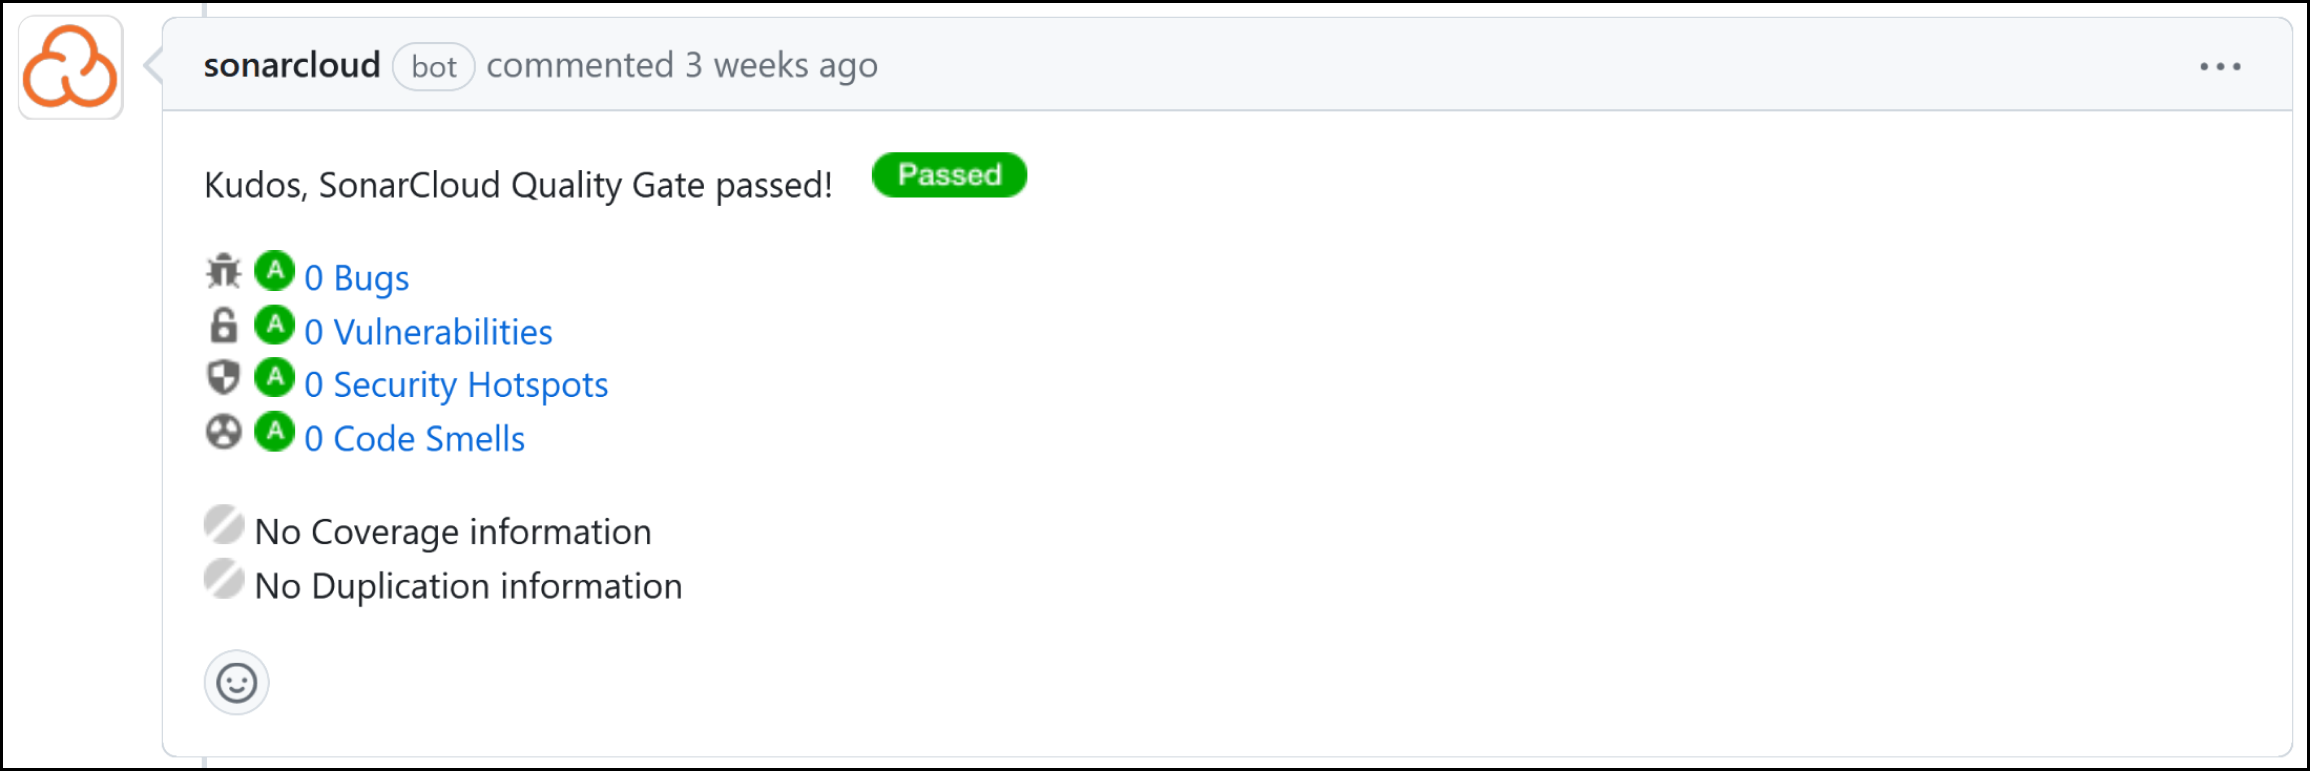
\includegraphics[width=12cm]{sonarcloud.png}
    \caption{\textit{SonarCloud} issue detector for pull request}
    \label{fig:sonarcloud}
\end{figure}

\begin{figure}[H]
    \centering
    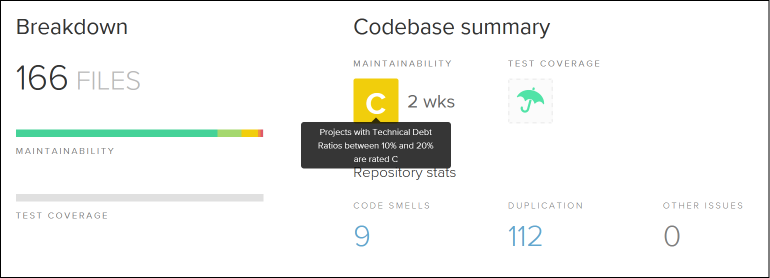
\includegraphics[width=12cm]{codeclimate.png}
    \caption{\textit{Code Climate} code base summary}
    \label{fig:codeclimate}
\end{figure}

\subsection{Tests}

The back- and frontend testing are crucial quality checkpoints, as a failure in either would prevent the deployment of the system (see Figure \ref{fig:tests}). Unit, integration, and UI tests have been implemented, but end-to-end tests have not been finalized. Testing of the onion architecture, as described in Section \ref{sec:subsystems}, was done using 39 unit tests. Additionally, 17 integration tests were employed to test the behavior of combined layers.

\begin{figure}[H]
    \centering
    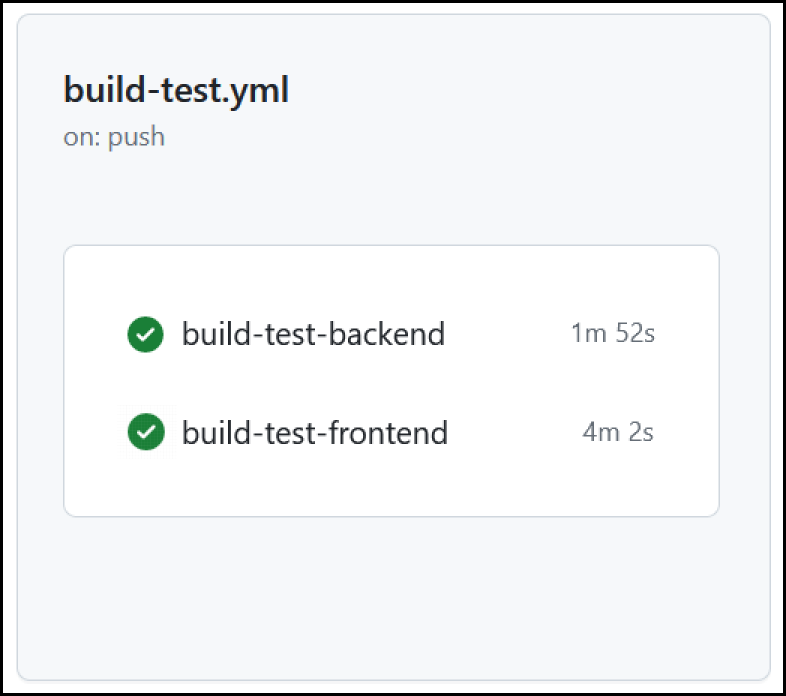
\includegraphics[width=5cm]{build-test.png}
    \caption{Chain of back- and frontend tests}
    \label{fig:tests}
\end{figure}

\section{Licence Compatability}
This project uses a MIT licence. This license is one of the most permissive licenses and therefore also compatible with other open source licenses \cite{wheeler:floss-license-slide}. 

\textbf{Show how the licenses are distributed using ScanCode - linux}

%no license found on Moq dependency


%license-checker --json > licenses.json

